\documentclass[twoside]{article}
\setlength{\oddsidemargin}{0.25 in}
\setlength{\evensidemargin}{-0.25 in}
\setlength{\topmargin}{-0.6 in}
\setlength{\textwidth}{6.5 in}
\setlength{\textheight}{8.5 in}
\setlength{\headsep}{0.75 in}
\setlength{\parindent}{0 in}
\setlength{\parskip}{0.1 in}

\usepackage{graphicx}
\usepackage{url}

%
% The following commands sets up the lecnum (lecture number)
% counter and make various numbering schemes work relative
% to the lecture number.
%
\newcounter{lecnum}
\renewcommand{\thepage}{\thelecnum-\arabic{page}}
\renewcommand{\thesection}{\thelecnum.\arabic{section}}
\renewcommand{\theequation}{\thelecnum.\arabic{equation}}
\renewcommand{\thefigure}{\thelecnum.\arabic{figure}}
\renewcommand{\thetable}{\thelecnum.\arabic{table}}
\newcommand{\dnl}{\mbox{}\par}

%
% The following macro is used to generate the header.
%
\newcommand{\lecture}[4]{
  \pagestyle{myheadings}
  \thispagestyle{plain}
  \newpage
  \setcounter{lecnum}{#1}
  \setcounter{page}{1}
  \noindent
  \begin{center}
  \framebox{
     \vbox{\vspace{2mm}
   \hbox to 6.28in { {\bf COMPSCI~590S~~~Systems for Data Science
                       \hfill Fall 2016} }
      \vspace{4mm}
      \hbox to 6.28in { {\Large \hfill Lecture #1: #2  \hfill} }
      \vspace{2mm}
      \hbox to 6.28in { {\it Lecturer: #3 \hfill Scribe(s): #4} }
     \vspace{2mm}}
  }
  \end{center}
  \markboth{Lecture {#1}: #2}{Lecture {#1}: #2}
  \vspace*{4mm}
}

%
% Convention for citations is authors' initials followed by the year.
% For example, to cite a paper by Leighton and Maggs you would type
% \cite{LM89}, and to cite a paper by Strassen you would type \cite{S69}.
% (To avoid bibliography problems, for now we redefine the \cite command.)
%
\renewcommand{\cite}[1]{[#1]}

% \input{epsf}

%Use this command for a figure; it puts a figure in wherever you want it.
%usage: \fig{NUMBER}{FIGURE-SIZE}{CAPTION}{FILENAME}
\newcommand{\fig}[4]{
           \vspace{0.2 in}
           \setlength{\epsfxsize}{#2}
           \centerline{\epsfbox{#4}}
           \begin{center}
           Figure \thelecnum.#1:~#3
           \end{center}
   }

% Use these for theorems, lemmas, proofs, etc.
\newtheorem{theorem}{Theorem}[lecnum]
\newtheorem{lemma}[theorem]{Lemma}
\newtheorem{proposition}[theorem]{Proposition}
\newtheorem{claim}[theorem]{Claim}
\newtheorem{corollary}[theorem]{Corollary}
\newtheorem{definition}[theorem]{Definition}
\newenvironment{proof}{{\bf Proof:}}{\hfill\rule{2mm}{2mm}}

% Some useful equation alignment commands, borrowed from TeX
\makeatletter
\def\eqalign#1{\,\vcenter{\openup\jot\m@th
 \ialign{\strut\hfil$\displaystyle{##}$&$\displaystyle{{}##}$\hfil
     \crcr#1\crcr}}\,}
\def\eqalignno#1{\displ@y \tabskip\@centering
 \halign to\displaywidth{\hfil$\displaystyle{##}$\tabskip\z@skip
   &$\displaystyle{{}##}$\hfil\tabskip\@centering
   &\llap{$##$}\tabskip\z@skip\crcr
   #1\crcr}}
\def\leqalignno#1{\displ@y \tabskip\@centering
 \halign to\displaywidth{\hfil$\displaystyle{##}$\tabskip\z@skip
   &$\displaystyle{{}##}$\hfil\tabskip\@centering
   &\kern-\displaywidth\rlap{$##$}\tabskip\displaywidth\crcr
   #1\crcr}}
\makeatother

% **** IF YOU WANT TO DEFINE ADDITIONAL MACROS FOR YOURSELF, PUT THEM HERE:



% Some general latex examples and examples making use of the
% macros follow.

\begin{document}

%FILL IN THE RIGHT INFO.
%\lecture{**LECTURE-NUMBER**}{**DATE**}{**LECTURER**}{**SCRIBE**}
\lecture{8}{Large-Scale Graph Analytics: Pregel and Arabesque}{Emery Berger}{Abhinav Khandelwa, Natcha Simsiri}

\section{Graph Analytics}
In today's age where linked data is ubiquitous - e.g. relationships in Social Networks, Topological
Information - graphs are often the go-to abstraction for modeling these types of data. The talk mainly focuses on the design methodology of parallel and distributed systems that does a variety of graph analytics as supposed to the design of graph algorithms themselves.
Three main types of graph systems are focused: 
1. Graph Computation and Search e.g. Pregel, TLV 
2. Graph Mining e.g. Arabesque

\section{Graph Computation and Search}
In graph computation you are given an input graph and you want to compute some updates on it. Page
Rank is the traditional problem in graph Computation. It is used by Google for page raking websites. In this
case web pages are the vertices and hyper links are the edges of the graph. We can represent this as 
an adjacency matrix where a cell encodes an edge, indices encode a vertex and computation is done by iteratively
transforming the matrix such that on termination, each vertex corresponds to a ranking.
Graph search tackles the problem of finding an instance of a subgraph or a path such that an invariant is maintained. 
Examples would be finding the shortest path or a bipartite graph.

\section{Pregel}
In Pregel, the input graph is its computational structure. Each vertex in the input graph is a thread that potentially computes a local state. Edges are stored as an adjacency list. So, each vertex has the the adjacency list for the
edges going to the neighboring vertex. In Pregel, the communication between two vertices is via messaging. 
Every vertex does some computation and pushes messages to the neighbous. Furthermore, distributed graph computation 
in Pregel is done by partitioning the input graph and handing each worker a partition of the graph. The Computation in Pregel goes
through bi synchronous programming paradigm. At every state each vertex computes new state based on
message received from previous states, then push the messages to next neighbors which passes through the
synchronous barrier.

\begin{figure}[ht]
  \centering
  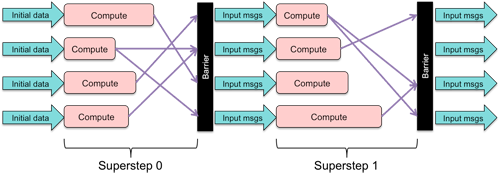
\includegraphics[width=0.7\linewidth]{Pregel-barrier-sync.png}
  \caption{Pregel: Barrier Synchronization}
  \vspace{-0.2cm}
  \label{fig:blockdiagram}
  \vspace{-0.2cm}
\end{figure}

 When a vertex completes its computation it calls for halt and when we have no more
active vertices the computation stops.
Another application of Pregel is in the Single Source Shortest Path. In this application we have graphs with
weighted edges. The output is the shortest distance of each vertex from the source vertex.

\begin{figure}[ht]
  \centering
  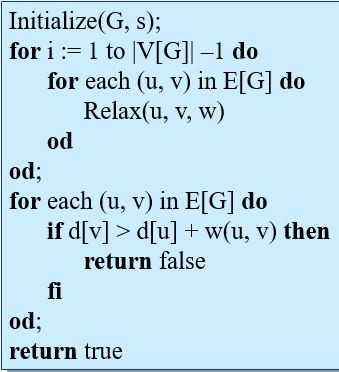
\includegraphics[width=0.7\linewidth]{BellmanFord-algorithm.jpg}
  \caption{Bellman Ford Single Source Shortest Path Algorithm}
  \vspace{-0.2cm}
  \label{fig:blockdiagram}
  \vspace{-0.2cm}
\end{figure}

If we were to do the same computation using MapReduce it will be as follows: There will be a file with multiple rows and each will have the attributes as vertex number, out adjacency etc. as shown in figure.
Every intermediate step will be written to this file as well.

\begin{figure}[ht]
  \centering
  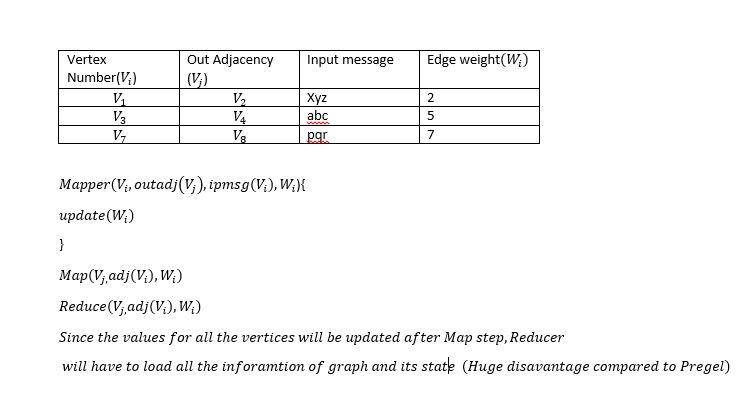
\includegraphics[width=0.7\linewidth]{MapReduce-on-SSSP.jpg}
  \caption{MapReduce on Single Source Shortest Path}
  \vspace{-0.2cm}
  \label{fig:blockdiagram}
  \vspace{-0.2cm}
\end{figure}

The issue with MapReduce is that it will send the same information over and over again to the reducer using network. The other issue is that MapReduce stores file in disk which are very slow to access compared to Pregel which stores messages in memory.

In pregel, Combiner is a technique to reduce the amount information sent over the networks by merging all the local messages to the same vertex. Aggregator is called on map key-value pair, each worker executes local aggregator which creates aggregation tree. First each worker aggregates the value then later mater aggregates all the values from the workers.

\section{Issues with Pregel}
While Pregel's parallelism is achieved within each "superstep" and "supersteps" are sequential with one another,
the time a "superstep" takes to complete is equivalent to the slowest vertex being processed. This means if one worker has lot more work to be done than other workers, the rest will have to wait - i.e we have a straggler. Similarly, if a few vertices is of higher degree than many others, we get a potentially network bottleneck or what is referred to as a hotspot. In fact, it turns out a lot of graphs in the real world are of this type:  the top 1 percent vertices are adjacent to 53 percent of the edges. They will create bottlenecks due to communication messages, storage, speed etc.

\section{Power graph}
Identify the hotsopts and replicate those high degree vertices. They use the idea of Gather, Apply and Scatter operation. These operation help in solving fan in problems. 

\section{Graph Mining} 
In graph mining we try to find the patterns of interests based on some properties. e.g. finding cliques in a graph - a subgraph where every vertex has an edge to every other vertex, motif counting - finding all subgraphs or embeddings that display connected patterns with induced-vertices, and and frequent sub-graph mining - counting subgraphs that are isomorphic to each other. 

Concept: you have an input graph and a pattern, i.e a sub-graph of the input graph, an embedding is defined as the sub-graph of the graph which matches a particular pattern - in other words, other instances of the subgraph that are isomorphic to the input pattern. Two graphs are isomorphic if there is a one-to-one function that maps each vertex and edge from one graph to the other graph. However, two embeddings are automorphic of they are isomorphic and each mapping is an identity mapping - i.e vertices and edges are the equivalent. This concept is very important since a lot of the time we are counting isomorphic graphs that are not automorphic.

In graph mining the fundamental problem is to do graph exploration and Arabesque is a pretty good at these tasks. Our goal is to enumerate subgraphs while checking for isomorphism between an embedding and a pattern, and at the same time prune and eliminate enumerated embeddings that are automorphic to already searched ones.

\section{Arabesque}
Arabesque is based on a think like a embedding paradigm which is proposed to be a better model for doing parallel and distributed graph mining as supposed to previously mentioned think like a vertex paradigm presented in Pregel. Similar to MapReduce and Pregel, code is very simple to write in Arabesque as it abstracts away most of the low level graph processing and distributed computation from user. At its core, Arabesque does automated subgraph exploration using user defined filter-process model as a guideline. First Arabesque takes an initial set of embedding and expands the embedding with respect the input graph resulting in candidate embeddings. Then the candidate embeddings are filtered through a user-defined call-back that satisfies the following: first, all automorphic embeddings must have the same filter results and second, if an embedding fails to satisfy the filter, the expansion of that embedding must also not satisfy the filter - this is called the anti-monotonicity property. Automorphism check gives Arabesque power to prune identical embeddings while the second ensures the correctness of quickly pruning a sub-graph of what it thinks will lead to an unsatisfiable embedding. Both these properties allow correct and efficient distributed graph mining. 

Here's an example of Arabesque's computational model: In clique finding example embedding will be taken as input and in the exploration process we will prune the sub-graphs which are not cliques and explore further with the interesting part of the graph. The reason of pruning is that a super graph of a sub-graph which is not a clique can never be a clique. Frequent graph mining is another problem that can be solved by Arabesque. Arabesque also works pretty good on a single thread application. Arabesque system does exploration,aggregation by pattern and load balancing which is abstracted away from user. 
  
\section{Arabesque's Implementation}

Arabesque is built on top of Giraffe, but only leverages Giraffe's distribution computation framework (as supposed to using its think like vertex graph processing model). Arabesque then distributes the same input graph to all workers to do sub-graph enumeration and filtering of embeddings such that communication between workers are is independent of the the input graph. This ensures that Arabesque does not get the same Hotspot problem as Pregel as problems like network congestion will no longer result from the structure of the graph. Arabesque utilizes the coordination-free exploration strategy to ensure that it will not enumerate on identical embeddings across all workers. This makes graph-mining highly paralell. Coordination-free exploration utilizes the previously stated invariants for filtering embedding as well as pruning canonical embeddings (a unique embedding, i.e no other canonical embedding is automorphic to the current one). Canonical embedding extendability ensures the correctness of such pruning method. Extendability is if a current embedding is found to be canonical, then next embedding (given an edge or vertex) must also be canonical. Arabesque makes sure this property holds by always traversing sub-graphs in an orderly fashion (ordered by vertex). We can think of this set of canonical embeddings as list of sorted canonical embedding by traversal order which as a result, checking whether an extension to an embedding is canonical is merely checking if there exists a canonical embedding in the list with the same prefix such that at the extension vertex's position contains a vertex id greater than the extended vertex's id. Implementation wise, canonical embeddings are stored as sort of a prefix DAG (What they call ODAG) where each "node" indicates the layer for ith vertices in the embedding - and each vertex in the layer has a pointer to the vertex in the next layer (as seen in  ODAG figure). This can be thought of as a compressed version of all canonical embeddings which achieves polynomial space as supposed to exponential space usage. 

The load balancing is done by round robin of distributing blocks of \b embeddings. 

\begin{figure}[ht]
  \centering
  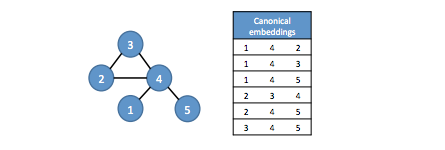
\includegraphics[width=0.7\linewidth]{embeddings}
  \caption{List of canonical embeddings in sorted order}
  \vspace{-0.2cm}
  \label{fig:blockdiagram}
  \vspace{-0.2cm}
\end{figure}

\begin{figure}[ht]
  \centering
  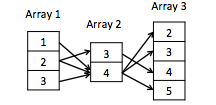
\includegraphics[width=0.7\linewidth]{odag}
  \caption{ODAG}
  \vspace{-0.2cm}
  \label{fig:blockdiagram}
  \vspace{-0.2cm}
\end{figure}

 
\end{document}